\section{Model-based Planner}
The model-based planner receives the ball’s position at each timestep and predicts the desired racket’s striking position, velocity, and timing. These predictions are then passed to the whole-body controller to generate robot motions.

\subsection{State Estimation}
\label{subsec:state_estimation}
Before predicting the ball’s trajectory, we first estimate its velocity, which cannot be directly obtained from the motion capture system. To do this, we perform a least-squares fit of a second-order polynomial to the ball’s position over time in each coordinate direction, $\mathbf{p}(t)=[p_x(t), p_y(t), p_z(t)]$. The fitting is performed using the nearest 31 position measurements, providing a smooth estimate of both position and velocity. Upon detecting a bounce on the table, we clear the position measurement buffer to prevent the inclusion of pre-bounce data. The smoothed value of the ball's position and velocity at the current timestep are then attained by evaluating $\mathbf{p}(t)$ and its derivative $\dot{\mathbf{p}}(t)$.

\subsection{Ball Trajectory Prediction}
To predict the ball trajectory, we adopt the same hybrid dynamics model as in~\cite{nguyen2025high}:

\begin{subnumcases}{\Sigma:\ }
  \mathbf{a} = -k \|\mathbf{v}\|\, \mathbf{v} + \mathbf{g}, & $\mathbf{p} \notin \mathcal{S}$, \label{eq:flight_dynamics}\\[6pt]
  \mathbf{v}^{+} = \mathbf{C}\,\mathbf{v}^{-},                        & $\mathbf{p} \in \mathcal{S}$,  \label{eq:bouncing_dynamics}
\end{subnumcases}
where~\eqref{eq:flight_dynamics} describes the continuous-time flight dynamics of the ball, with $\mathbf{a}$ and $\mathbf{v}$ denoting its acceleration and velocity, respectively. 
Here, $k$ is the aerodynamic drag coefficient and $\mathbf{g}$ is the gravity vector. 
We assume the spin is sufficiently small so that spin-induced effects, such as the Magnus force, can be neglected. Equation~\eqref{eq:bouncing_dynamics} models the discrete-time impact dynamics upon bouncing on the table, where $\mathbf{v}^-$ and $\mathbf{v}^+$ represent the pre- and post-impact velocities. 
The restitution matrix is
\begin{equation}
    \mathbf{C} = \mathrm{diag}(C_h,\, C_h,\, -C_v),
\end{equation}
with $C_h$ and $C_v$ denoting the horizontal and vertical restitution coefficients, respectively. The set of impact states is
\begin{equation}
    \mathcal{S} = \bigl\{\, \mathbf{p} = [p_x,\,p_y,\,p_z] \;\big|\; p_z = 0 \,\bigr\}.
\end{equation}

\begin{figure}
    \centering
    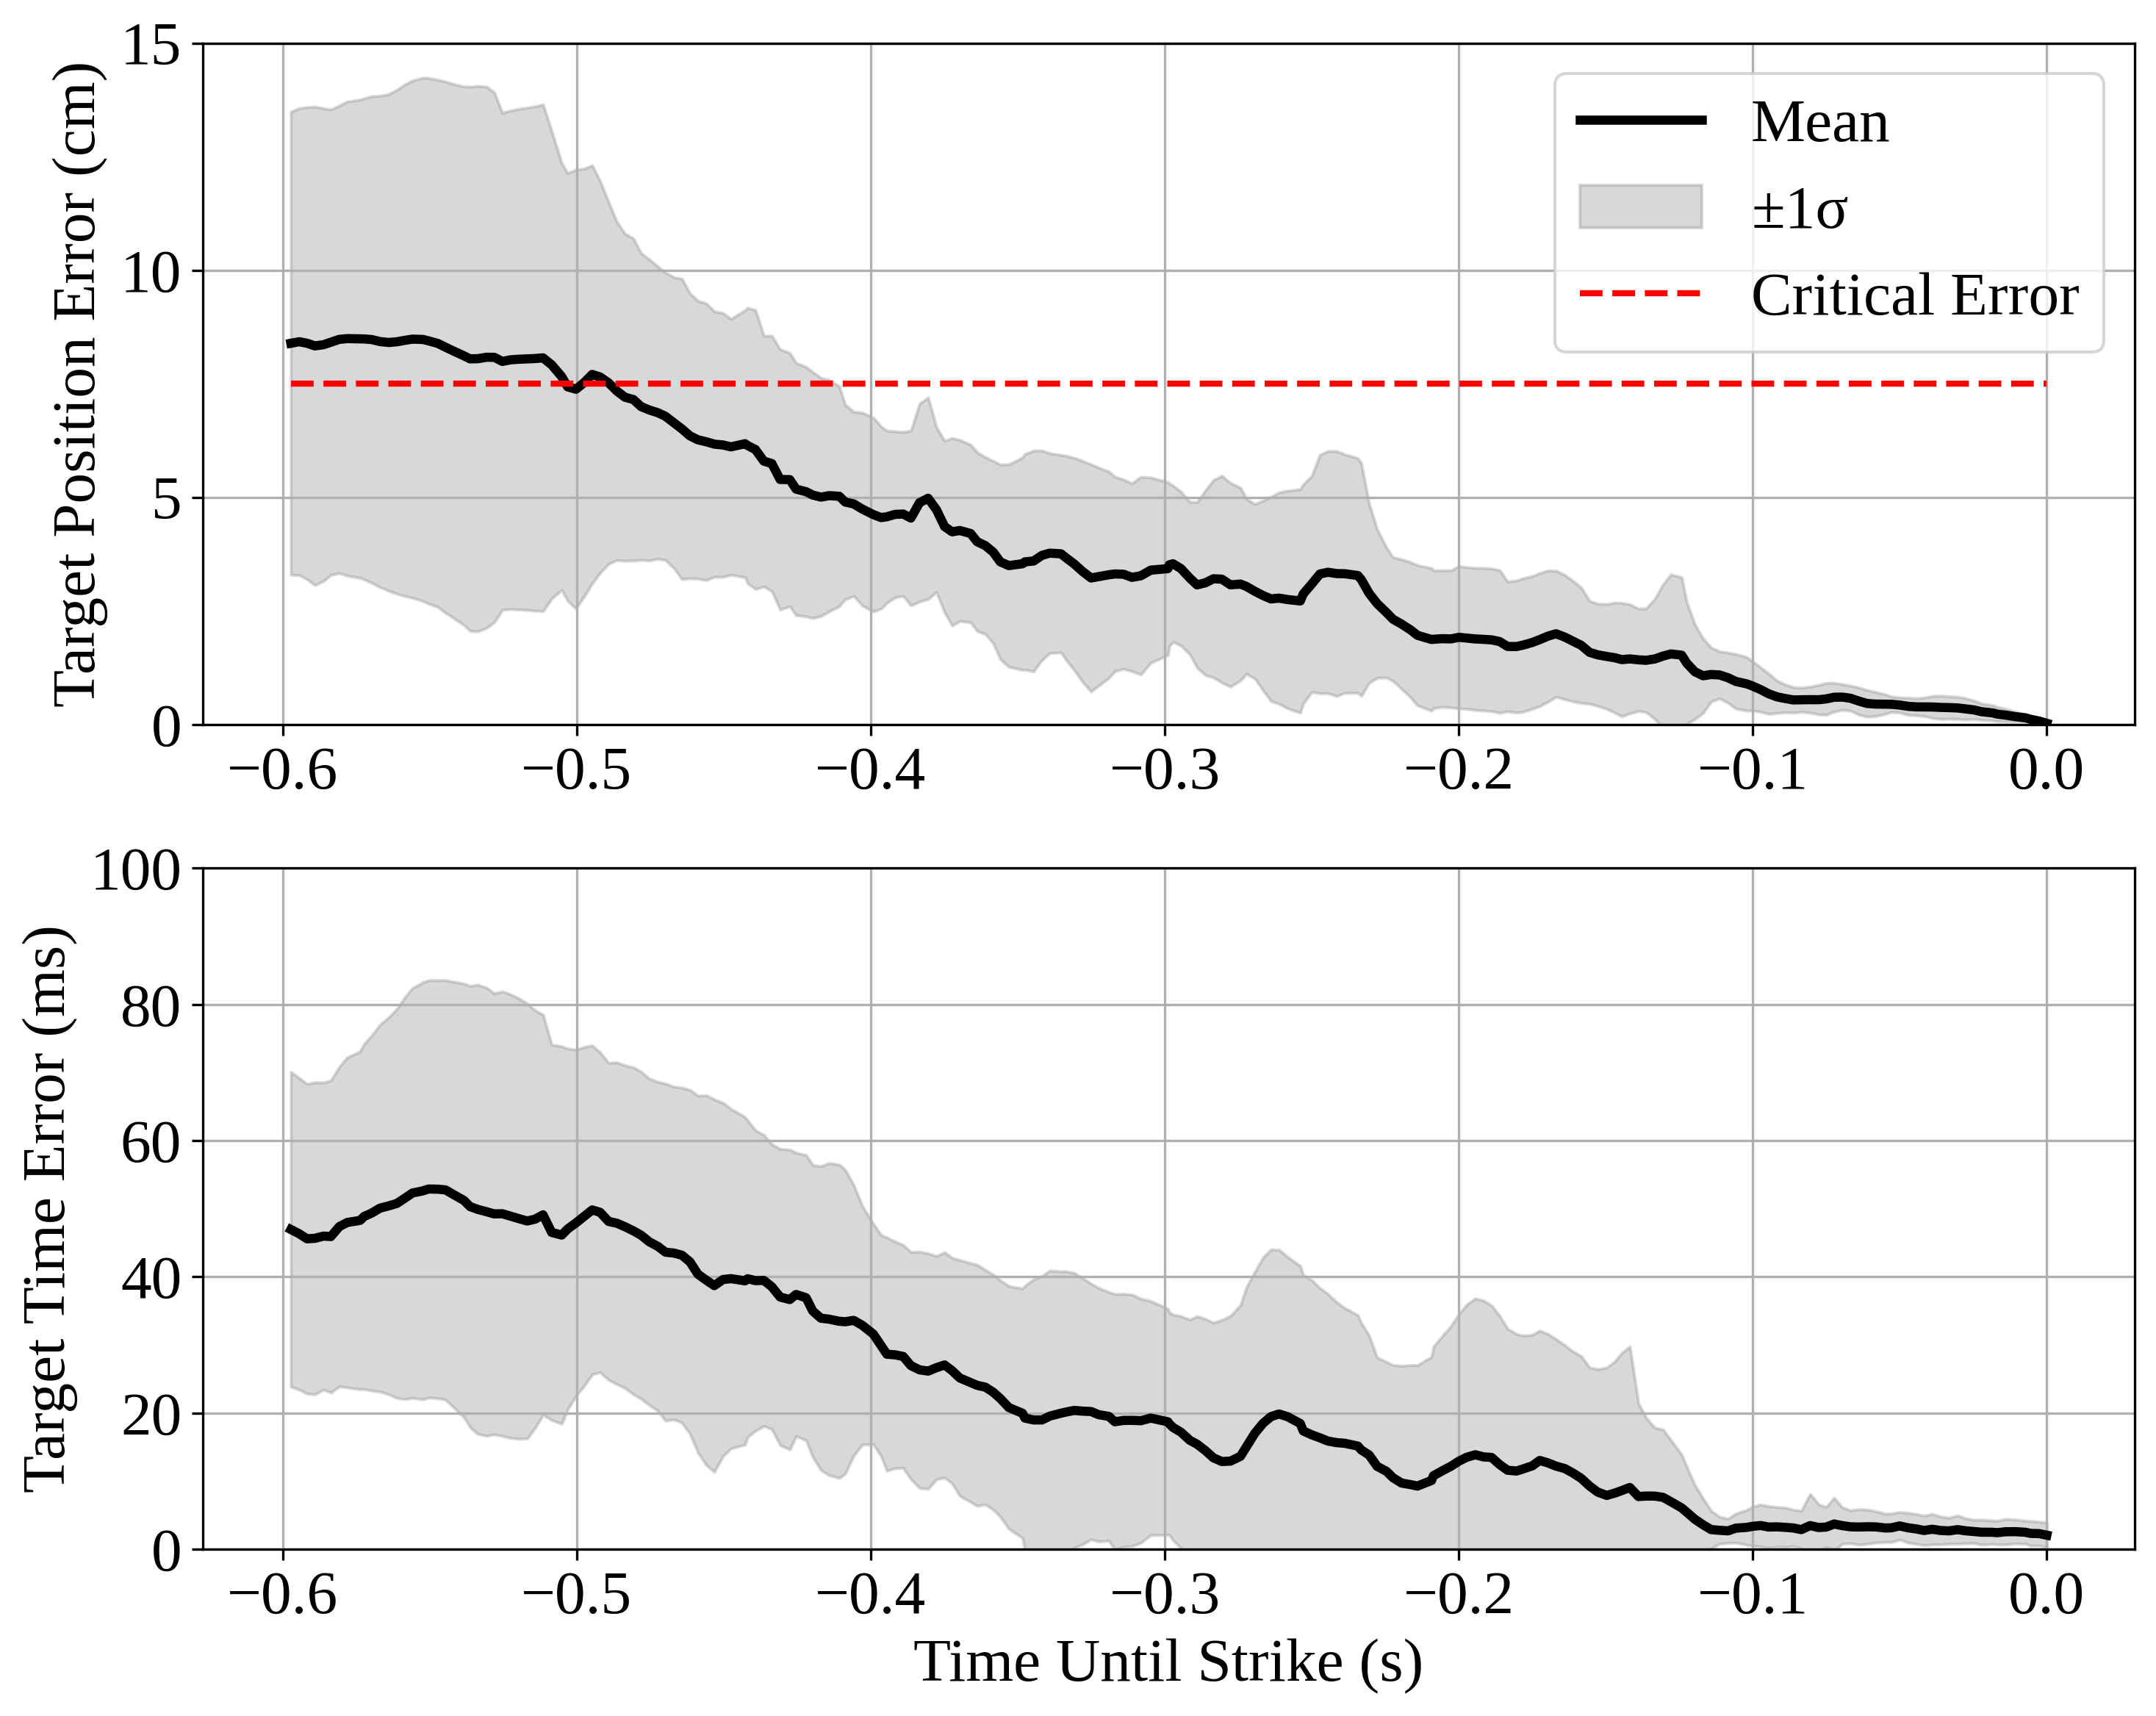
\includegraphics[width=1\linewidth]{figures/prediction_error.png}
    \caption{\textbf{Prediction errors of the model-based planner.} Striking position error (top) and striking time error (bottom) are evaluated over 20 ball trajectories. The shaded regions indicate the standard deviation, and the red dashed line marks the critical position error of 7.5\,cm, corresponding to the racket radius. At 0.5\,s before the strike, the position error falls below this threshold.}
    \label{fig:prediction_error}
\end{figure}


We estimate the parameters $k$, $C_h$, and $C_v$ from 15 recorded ball trajectories. 
In each trajectory, the ball is launched from one side of the table, bounces once on the opposite side, and then exits the table. 
The parameters are identified by fitting the recorded data to the following:
\begin{equation}
\begin{cases}
\|\mathbf{a}-\mathbf{g}\| = k\|v\|^2, \\
\{\|v_x^+\|, \|v_y^+\|\} = C_h \{\|\{v_x^-\|, \|v_y^-\|\}, \\
\|v_z^+\| = C_v \|v_z^-\|, \\
\end{cases}
\label{eq:fit_eqs}
\end{equation}
where $\mathbf{v}$ and $\mathbf{a}$ are estimated from the first and second derivatives of $p(t)$, respectively. Using this model, we apply explicit step-by-step time integration to predict the ball’s future position and velocity, initialized with the estimates from Sec.~\ref{subsec:state_estimation}. Given a predefined virtual hit plane~\cite{mulling2010biomimetic, mulling2011biomimetic, kocc2018online} at $x = -1.37\,\mathrm{m}$, the corresponding hitting time and position can then be computed.

\begin{figure}
    \centering
    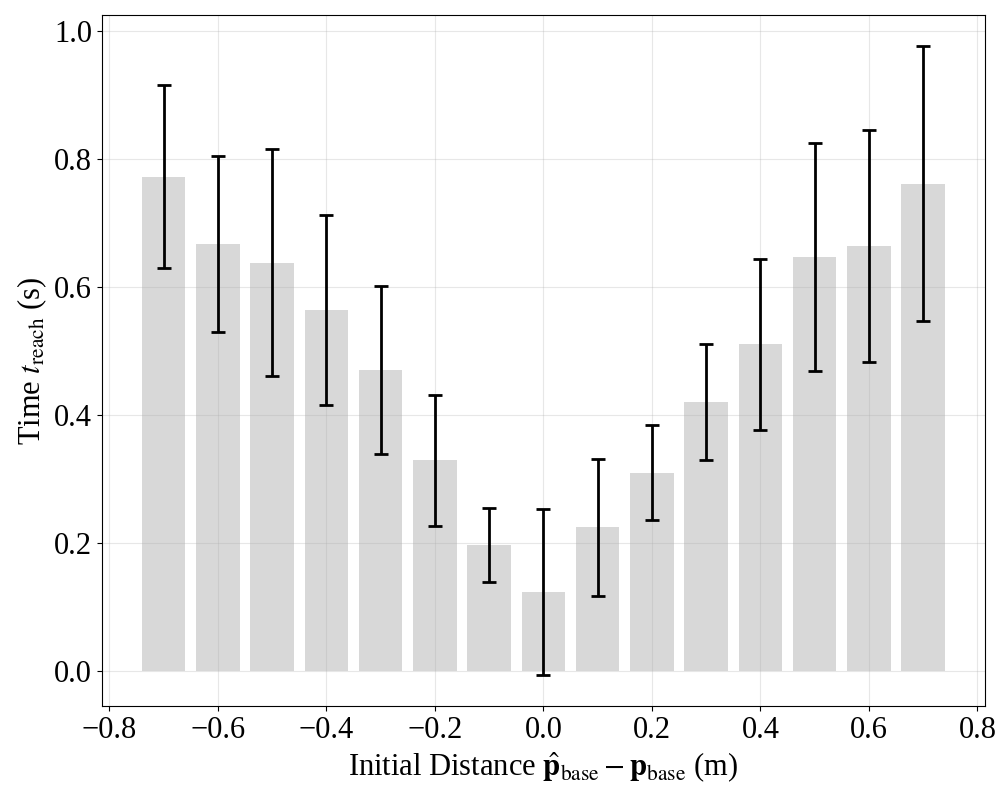
\includegraphics[width=1\linewidth]{figures/agility_test.png}
    \caption{\textbf{Agility evaluation of the WBC policy.} Based on 943 successful simulated trials (94.3\% success rate), when the initial distance is within 0.75\,m, the target can be reached in under 0.8\,s on average, which is faster than the strike time of 0.86\,s. Error bars denote standard deviation across trials.}
    \label{fig:agility_test}
\end{figure}


\subsection{Racket-ball Interaction}
In addition to making contact with the ball, our objective is to successfully return it, which requires determining the racket’s orientation and velocity at the moment of impact. We assume that, at impact, the racket plane is perpendicular to its velocity vector. Unlike approaches that aim to precisely control the landing position, our goal is to ensure a valid return. Thus, we adopt a simplified post-impact flight model and racket-ball interaction model.

During racket-ball contact, we assume a coefficient of restitution $C_r$ along the normal to the racket surface and neglect tangential friction. After impact, the ball is assumed to be subject only to gravity during flight. Given the desired landing position on the table $\hat{\mathbf{p}}_l$, the desired hitting position $\hat{\mathbf{p}}_{\mathrm{racket}}$, and a predefined flight time from hitting to landing $\Delta t$, the desired outgoing ball velocity $\mathbf{v}_o$ is computed as:
\begin{equation}
\mathbf{v}_o=\dfrac{\hat{\mathbf{p}}_l-\hat{\mathbf{p}}_\mathrm{racket}}{\Delta t}+\frac{1}{2}\mathbf{g}\Delta t,
\end{equation}
where $\hat{\mathbf{p}}_l$ is set to the center of the opponent’s side of the table. Based on the desired outgoing velocity $\mathbf{v}_o$ and the predicted incoming velocity $\mathbf{v}_i$, the desired racket velocity $\hat{\mathbf{v}}_{\mathrm{racket}}$ can be computed as:
\begin{equation}
\hat{\mathbf{v}}_{\mathrm{racket}} = \dfrac{\mathbf{v}_o\cdot\mathbf{u}+C_r \mathbf{v}_i\cdot\mathbf{u}}{1+C_r}\mathbf{u},
\end{equation}
where $\mathbf{u}=\dfrac{\mathbf{v}_o - \mathbf{v}_i}{\|\mathbf{v}_o - \mathbf{v}_i\|}$ is the unit vector in the direction of $\mathbf{v}_o - \mathbf{v}_i$. 
The desired racket velocity, together with the predicted hitting position and time, is then passed to the learning-based whole-body controller, which generates the corresponding robot motion.
